\documentclass[tikz,border=2mm]{standalone}
\usepackage{tikz}
\usepackage{tikz-feynman}
\tikzfeynmanset{compat=1.1.0}

\begin{document}

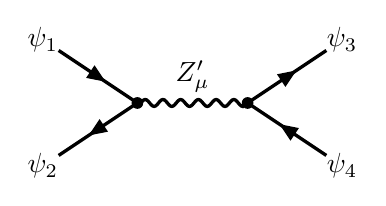
\begin{tikzpicture}
\begin{feynman}
    % Vertici principali
    \vertex [inner sep=0pt](i1) at (0,0.8) {$\psi_1$};
    \vertex [inner sep=0pt](i2) at (0,-0.8) {$\psi_2$};
    \vertex [inner sep=0pt](v1) at (1.2,0) {};
    \vertex [inner sep=0pt](v2) at (2.6,0) {};
    \vertex [inner sep=0pt](f1) at (3.8,0.8) {$\psi_3$};
    \vertex [inner sep=0pt](f2) at (3.8,-0.8) {$\psi_4$};

    % Marker visibili
    \node[circle, fill=black, inner sep=1.5pt] at (v1) {};
    \node[circle, fill=black, inner sep=1.5pt] at (v2) {};

    % Diagramma
    \diagram* {
        (i1) -- [fermion,line width=1.2pt] (v1) -- [fermion,line width=1.2pt] (i2),
        (v1) -- [boson, edge label=$Z^\prime_\mu$,line width=1.2pt] (v2),
        (v2) -- [fermion,line width=1.2pt] (f1),
        (f2) -- [fermion,line width=1.2pt] (v2),
    };
\end{feynman}
\end{tikzpicture}


\end{document}

% pdflatex feynman_diag.tex

% pdftoppm -png -r 300 tree-vector-s-channel.pdf tree-vector-s-channel
